\documentclass[UTF8,a4paper]{ctexart}
\usepackage[margin=1in]{geometry}

\usepackage{amsmath}
\usepackage{amssymb}
\usepackage{graphicx}
\usepackage{anyfontsize}
\usepackage{siunitx}
\usepackage{hyperref}
\usepackage{booktabs}
\usepackage{multirow}

\title{FAIML Lab1 实验报告：使用线性模型探究 LLM 的内部表征}
\author{林思睿 PB24000301}
\date{2026 年 9 月 30 日}

\begin{document}
\maketitle

\begin{abstract}
本报告回答实验文档的 9 道思考题。核心工作包括：(1) 手写全批量梯度下降实现线性/逻辑回归
（含 $\ell_1$ 次梯度与 $\ell_2$ 正则），代码在 \texttt{model.py}；
(2) 用系数路径与一个可控案例分别说明 $\ell_1$/$\ell_2$ 的稀疏性质差异；
(3) 与 \texttt{sklearn} 在同一正则化语义下对比，验证实现正确；
(4) 对 world（地理坐标）与 truth（句子真假）两个线性探测任务做层数与正则化的
粗网格+细网格搜索，提交 \texttt{results/world.npz}（第 11 层）与
\texttt{results/truth.npz}（第 23 层），验证集指标分别为
坐标平均 MSE$=149.64$（纬度 MSE $=29.14$、经度 MSE $=270.13$，
两者的和 $299.27$ 是\emph{“纬度 MSE + 经度 MSE”}，不是 MSE）与准确率 $0.8833$；
(5) 对两个数据集的训练/验证分布差异做了定量分析，并给出可视化与基线对照。
\end{abstract}

\tableofcontents

%=============================================================
\section{思考题}

%-------------------------------------------------------------
\subsection{思考题 1：重现 $\ell_1$、$\ell_2$ 正则化的系数路径}

\paragraph{数据来源}
路径是在本实验自己的数据上画的：取 world 任务第 11 层表征的全部 $N=500$ 条训练样本，
按方差从 2560 维中选出数值最大的 8 维作为“可控的 8 特征”子问题，目标取纬度。
由于不同特征量纲差异大，特征与目标都做了 z-score 标准化，这样 $\lambda$ 对
$\ell_1$、$\ell_2$ 两条路径才有可比性（同一 $\lambda$ 表示同样的惩罚尺度）。
脚本：\texttt{coef\_path.py}；$\lambda\in[10^{-3},10^{1.5}]$ 共 45 个对数等距点。

\paragraph{求解方式}
$\ell_2$ 路径直接用 \texttt{model.py} 的梯度下降求解，并与闭式解
$(X^\top X/N+\lambda_2 I)^{-1}X^\top y/N$ 核对，路径末端与闭式解最大偏差
$2.6\times10^{-18}$，说明手写 GD 确实收敛到最优。
$\ell_1$ 路径若也用次梯度 GD，会在零点附近振荡、得不到精确的 $0$（实测在
$\lambda=31.6$ 时损失停在 $2.3$，而最优值应为 $1.0$），因此画路径时对 $\ell_1$
项改用近端算子（软阈值），即 ISTA 近端梯度下降，平滑项梯度与步长
$1/L$、$L=\lambda_{\max}(2X^\top X/N)$ 的取法与讲义一致。
\texttt{model.py} 中的训练仍严格按讲义使用次梯度（提交代码不受影响）。

\begin{figure}[htbp]
  \centering
  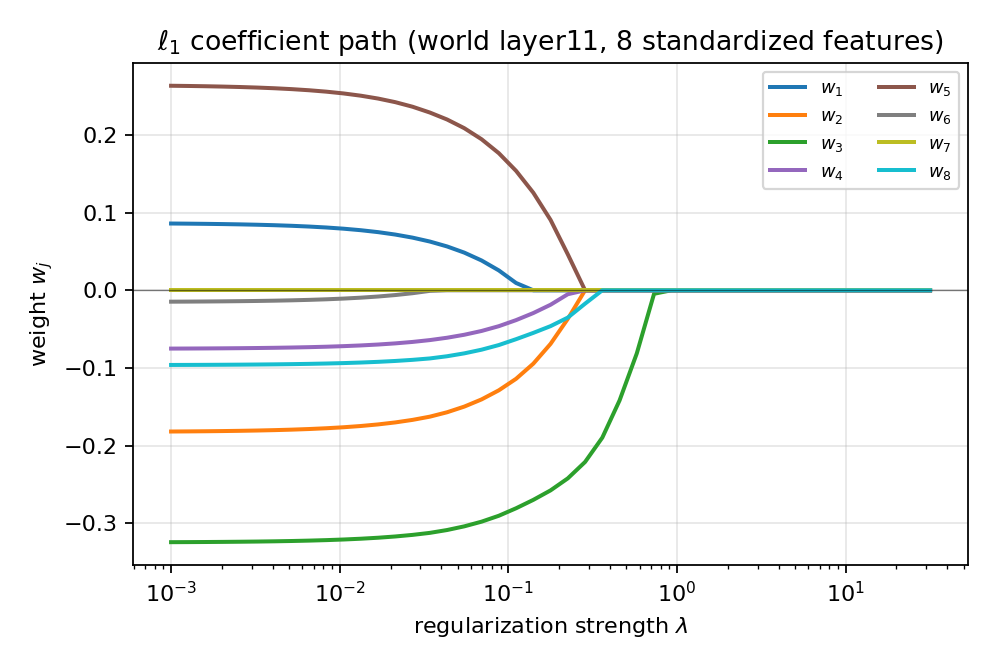
\includegraphics[width=0.48\textwidth]{figures/coef_path_l1.png}
  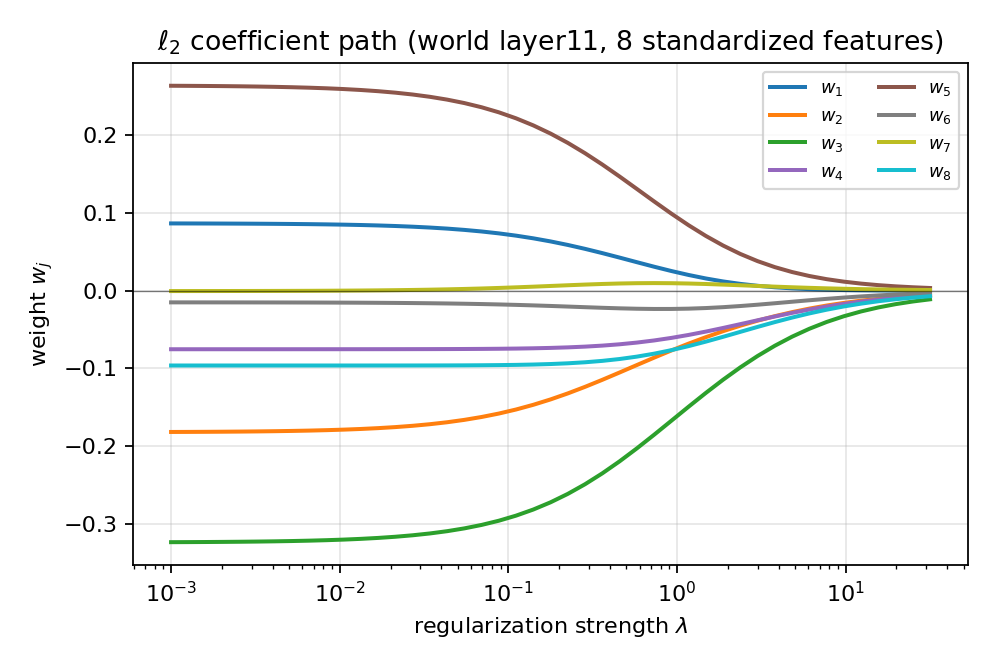
\includegraphics[width=0.48\textwidth]{figures/coef_path_l2.png}
  \caption{左：$\ell_1$ 系数路径（分段线性，随 $\lambda$ 增大出现精确的 0）；
  右：$\ell_2$ 系数路径（连续光滑收缩，永不为 0）。}
\end{figure}

\paragraph{观察}
$\ell_1$ 路径是分段线性的，随 $\lambda$ 增大被压成 0 的系数个数依次为
$[1,1,1,1,2,2,6,7,8,8,8,8]$（沿路径每 4 个点采样），即依次“剔除”贡献小的特征；
$\ell_2$ 路径上所有系数同时平滑收缩，在最大 $\lambda$ 处仍有非零值
（末端 $[0,-0.0055,-0.0112,-0.0061,0.0034,-0.0033,0.0008,-0.0072]$ 量级的
小系数），永远无法据此做特征取舍。

%-------------------------------------------------------------
\subsection{思考题 2：$\ell_2$ 用“把小系数设为 0”做特征选择是不好的}

\paragraph{案例构造}
脚本 \texttt{feature\_selection\_demo.py} 构造 18 维回归数据：$x_1,x_2,x_3$ 是真信号
（系数 $3,2,-1$），$x_6=0.95x_1+\varepsilon$、$x_7=0.95x_2+\varepsilon$ 是强相关副本
（现实中“两个高度相关特征携带同一信息”的常见情形），其余 13 维为纯噪声，
$y=Xw+\varepsilon$，噪声标准差 0.5。数据用一个固定种子生成后\emph{确定性}地切成
训练/验证/测试三份（各 300 条），\textbf{测试集全程不参与任何选择}。

\paragraph{比较口径}
若各自取“验证 MSE 最小”的 $\lambda$，两者都倾向于保留几乎所有特征（都还很小），
无法体现差异。因此额外给出\textbf{“稀疏口径”}：在验证 MSE 不超过各自最优值
$5\%$ 的 $\lambda$ 中取最大的那个，即“在几乎不损失预测精度的前提下尽量稀疏”，
再比较非零系数个数。$\lambda$ 与稀疏口径都只在验证集上确定，选定后才在
留出的测试集上评估一次最终 MSE，避免用测试集调参的选择泄漏。
$\ell_1$ 用 ISTA 精确求解，$\ell_2$ 用 \texttt{model.py} 的 GD。

\begin{table}[htbp]
\centering
\caption{$\ell_1$ 与 $\ell_2$ 在同一数据、同一 $\lambda$ 口径下的对比。
$\lambda$ 与稀疏口径均由验证集选定，测试 MSE 为选定后在留出测试集上的一次评估。}
\label{tab:fs}
\begin{tabular}{lcc}
\toprule
 & $\ell_1$ & $\ell_2$ \\
\midrule
最优（验证 MSE 最小）$\lambda$ & 0.03707 & 0.001 \\
\quad 对应验证 MSE & \textbf{0.2507} & 0.2562 \\
\quad 对应留出测试 MSE & \textbf{0.2341} & 0.2384 \\
稀疏口径 $\lambda$ & 0.1126 & 0.009237 \\
\quad 对应验证 MSE & 0.2573 & 0.2672 \\
\quad 对应留出测试 MSE & 0.2432 & 0.2445 \\
\quad 非零系数个数（真实支撑集 = 3） & \textbf{4} & 18 \\
\quad 恢复的支撑集 & $\{0,1,2,5\}$ & $\{0,\dots,17\}$ \\
\quad 纯噪声特征最大 $|w_j|$ & \textbf{0.0000} & 0.0494 \\
\quad 相关副本最大 $|w_j|$ & 0.0198 & 0.2762 \\
\quad $x_1$ 与 $x_6$ 上的权重 & 2.931 / 0.020 & 2.717 / 0.276 \\
\bottomrule
\end{tabular}
\end{table}

\begin{figure}[htbp]
  \centering
  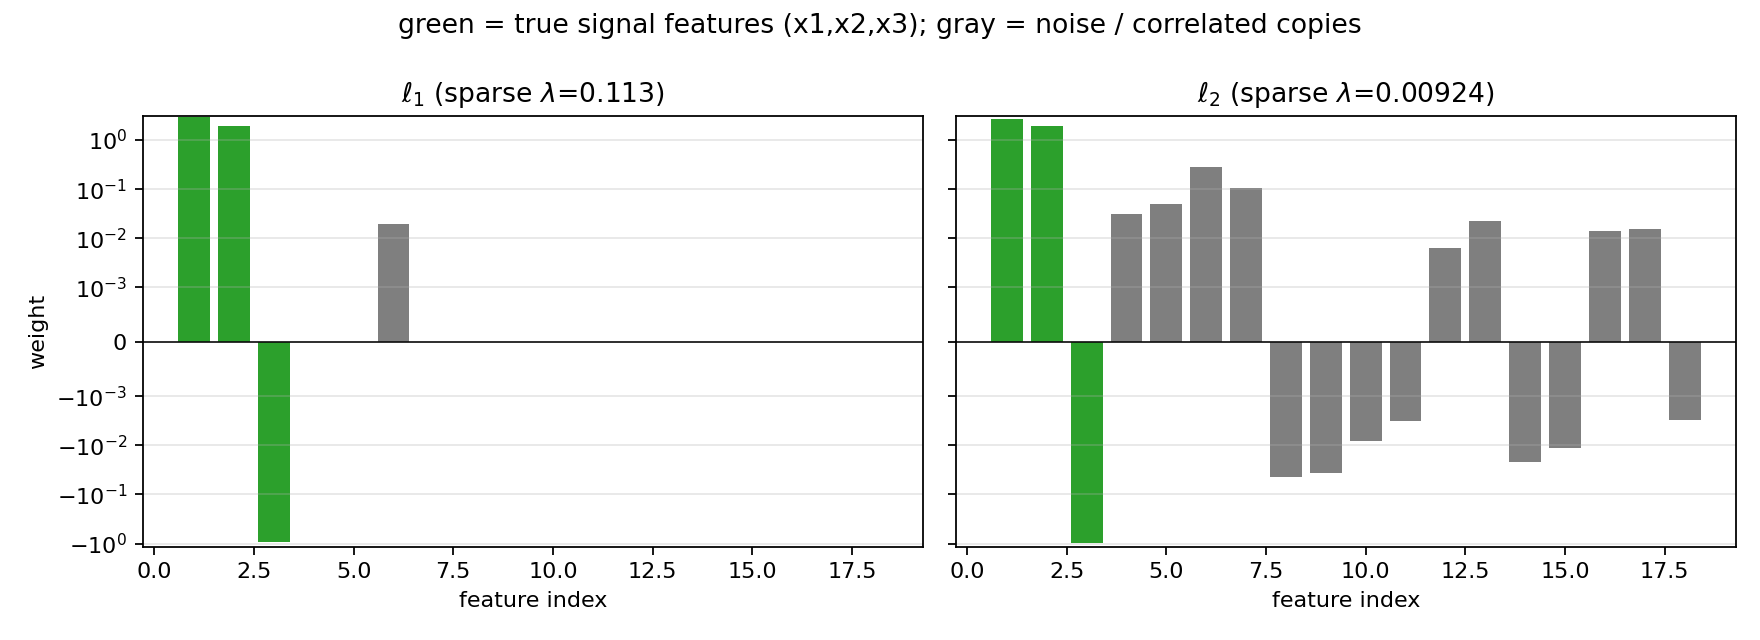
\includegraphics[width=0.85\textwidth]{figures/feature_selection_l1_l2.png}
  \caption{稀疏口径下两者的权重（绿色为真实信号特征）。$\ell_1$ 把纯噪声精确置 0，
  $\ell_2$ 的权重全部非零。}
\end{figure}

\paragraph{结论}
(1) $\ell_2$ 惩罚的是 $\sum w_j^2$，其最优解只会\emph{趋近} 0 而不会\emph{等于} 0，
任何“把小系数当 0”的判断都必须人为定阈值，而阈值没有客观标准，随量纲、
样本数变化就会失效；
(2) 更糟的是 $\ell_2$ 在相关特征之间\emph{平摊}权重（稀疏口径下 $x_1$ 与 $x_6$
分到 2.717/0.276，两者都被保留），于是“小”不代表“无用”，阈值一砍可能砍掉成对信息中的一半；
(3) $\ell_1$ 的解天然稀疏：在同一精度口径下纯噪声全部为 0，且留出测试 MSE
反而更小（最优口径 0.2341 $<$ 0.2384，稀疏口径 0.2432 $<$ 0.2445），
即更好的预测 + 可解释的特征子集，
这正是课件第 44 页强调 $\ell_1$ 适合特征选择的原因。

%-------------------------------------------------------------
\subsection{思考题 3：与 sklearn 实现的拟合效果差异}

脚本 \texttt{compare\_sklearn.py}。先明确换算关系（我们的目标函数按讲义
是\emph{平均}损失）：
\[
\text{回归：}\ \|Xw-y\|_2^2/N+\lambda_2\|w\|^2
\quad\Longleftrightarrow\quad
\texttt{Ridge}(\alpha=N\lambda_2)
\]
\[
\text{分类：}\ \operatorname{mean}(NLL)+\lambda_2\|w\|^2
\quad\Longleftrightarrow\quad
\texttt{LogisticRegression}\bigl(C=\tfrac{1}{2N\lambda_2}\bigr)
\]

\begin{table}[htbp]
\centering
\caption{与 \texttt{sklearn} 的对比结果。}
\label{tab:sk}
\small
\begin{tabular}{llcc}
\toprule
任务 & 指标 & 我们 & \texttt{sklearn} \\
\midrule
小例子（8 条、2 维，无正则） & 权重最大差 & \multicolumn{2}{c}{$9.99\times10^{-16}$} \\
world 第 11 层，原始特征 & 验证 MSE（纬度） & 29.1406 & 29.2737 \\
 & 验证 MSE（经度） & 270.1299 & 271.6993 \\
 & 训练目标 $J$ 差 & \multicolumn{2}{c}{$+0.161$ / $+0.324$（GD 未完全收敛）} \\
world 第 11 层，特征标准化 & 权重最大差 & \multicolumn{2}{c}{$1.05\times10^{-14}$ / $9.95\times10^{-14}$（纬/经）} \\
truth 第 23 层（$\lambda_2=0.03$） & 训练/验证准确率 & 0.9381 / 0.8833 & 0.9379 / 0.8833 \\
 & $\cos(w)$ / 权重最大差 & 0.999999 / $1.27\times10^{-4}$ & --- \\
 & 概率最大差 / 类别不一致 & $1.07\times10^{-3}$ / 0 条 & --- \\
\bottomrule
\end{tabular}
\end{table}

\paragraph{结论}
拟合效果\textbf{没有实质差异}：小例子与标准化后权重完全一致（$10^{-14}$ 量级），
truth 任务两边验证准确率相同（0.8833）、概率最大差 $10^{-3}$、无一条预测类别不同。
原始特征上 world 的权重最大差约 $0.25$（$\cos=0.995$），但验证 MSE 反而略优
（29.14 vs 29.27）。原因是 $N=500 \ll D=2560$，且特征均值不为零时存在
“权重与偏置相互抵消”的近零曲率方向（实测该方向的 Hessian 特征值小到
$\sim10^{-4}$），全批量 GD 在有限步内收敛慢，而 \texttt{sklearn} 用
\texttt{cholesky/SVD} 直接解正规方程。也就是说，差异来自\textbf{求解器的收敛
速度与数值路径}，而不是目标函数或正则化语义不一致。

%-------------------------------------------------------------
\subsection{思考题 4：不同层中间表征的预测效果对比与选层}

\paragraph{实验设置}
\texttt{sweep.py} 对每层独立做“粗网格 $\to$ 细网格”的 $\lambda$ 搜索，并比较
验证集上\emph{纬度 MSE + 经度 MSE} 之和（选层选参用的就是这个和，
各层对应的逐坐标平均 MSE 为它的一半）；
纬度、经度是两个独立的一维回归，分别取各自最优 $\lambda$（平方损失下
$n$ 维回归等价于 $n$ 个一维回归，见讲义 2.2 节）。

\begin{table}[htbp]
\centering
\caption{world 任务：各层在相同 $\lambda$ 下的\emph{“纬度 MSE + 经度 MSE”}之和
（注意这是两项 MSE 相加，不是 MSE），以及各层调参后的最好结果。}
\label{tab:layer_world}
\begin{tabular}{lcccc}
\toprule
$\lambda_2$ & 第 11 层 & 第 23 层 & 第 35 层 \\
\midrule
0（不加正则） & 789.17 & 683.36 & 664.11 \\
0.01 & 545.20 & 612.48 & 660.90 \\
0.05 & \textbf{376.33} & 510.73 & 648.67 \\
0.1 & \textbf{329.27} & 472.08 & 634.64 \\
0.5 & \textbf{308.63} & 452.67 & 556.20 \\
1.0 & \textbf{349.29} & 471.72 & 502.26 \\
\midrule
各层最优 $\lambda$（纬/经） & \textbf{0.14 / 0.28} & 0.2 / 0.28 & 2.0 / 2.0 \\
\quad 各层最好“纬度 MSE + 经度 MSE” & \textbf{299.27} & 447.98 & 449.13 \\
\quad （纬度 MSE / 经度 MSE） & (29.14/270.13) & (60.36/387.62) & (41.33/407.80) \\
\bottomrule
\end{tabular}
\end{table}

\begin{figure}[htbp]
  \centering
  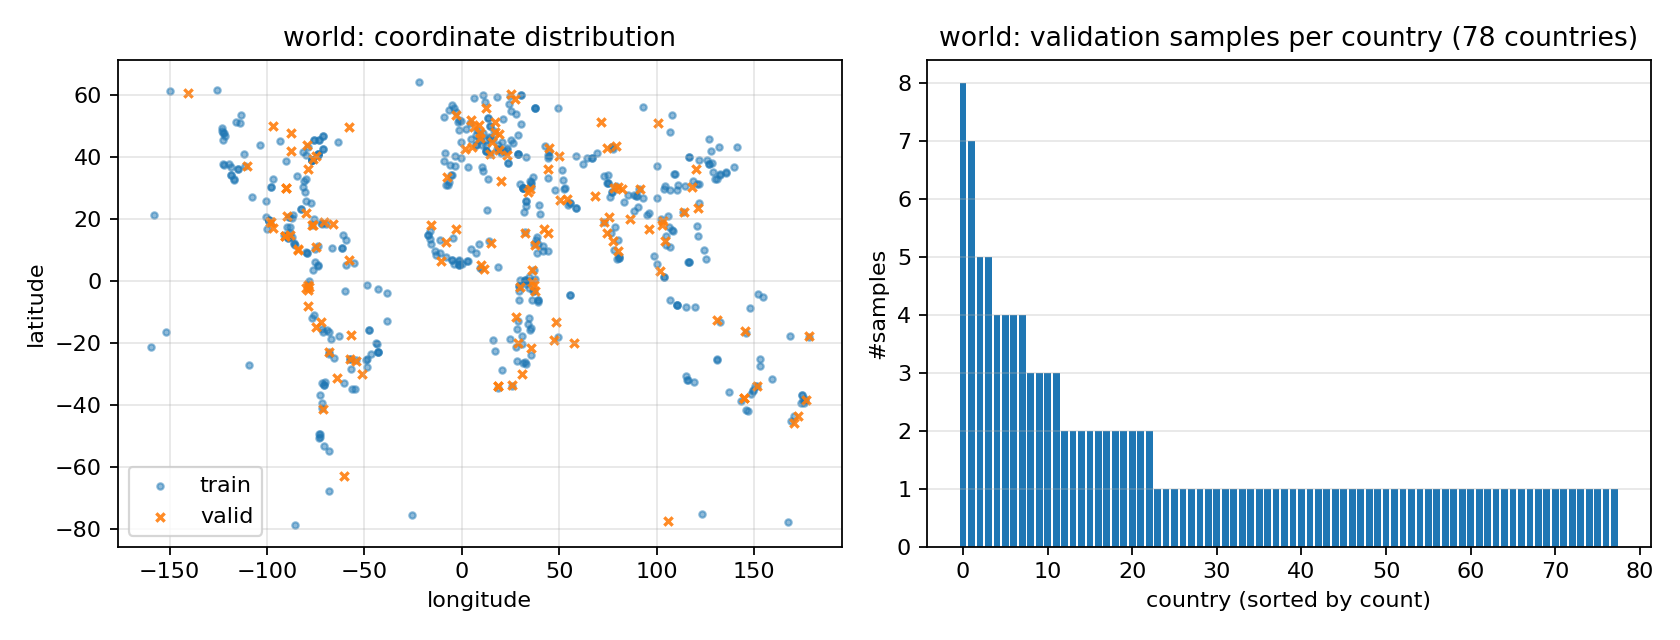
\includegraphics[width=0.75\textwidth]{figures/dist_world.png}
  \caption{world 训练/验证集的分布对照（坐标分布、表征范数、常数/国家均值基线等）。}
\end{figure}

\paragraph{原因分析}
\begin{enumerate}
  \item \textbf{在任何正则化水平下第 11 层都最好}（$\lambda_2\ge0.05$ 时明显领先），
  且各层调参后的“纬度 MSE + 经度 MSE”之差 299.27 vs 447.98/449.13，
  差距接近 50\%，不是调参噪声。
  \item \textbf{深层表征的尺度与均值剧烈增长}：训练集表征范数为
  $42.1\pm1.5$（L11）、$102.9\pm6.3$（L23）、$824.7\pm80.7$（L35），
  特征均值向量范数 $42.7/109.1/599.8$。深层的输入尺度大得多，
  同一个 $\lambda$ 在不同层含义完全不同（因此必须逐层选 $\lambda$），
  而它需要的强正则（第 35 层最优 $\lambda=2.0$）本身就会损失信息。
  \item 各层“单个特征与坐标的最大相关”其实接近：
  第 11/23/35 层纬度最大 $|r|$ 为 0.644/0.576/0.582，
  经度为 0.572/0.592/0.656，
  说明差距不来自某个超强单特征，而来自\textbf{多特征组合的泛化}：
  $N=500\ll D=2560$ 时，深层更偏向训练集里出现过的国家/地点模式，
  在 130 条验证样本（含 19 个训练未见国家）上更容易过拟合——
  这一点在 $\lambda=0$ 时最明显：第 11 层不加正则反而最差（789.17），
  说明它的可拟合（也即易过拟合）方向最多。
\end{enumerate}

\paragraph{最终选层}
按“每层独立调 $\lambda$ 后比较验证集上\emph{纬度 MSE + 经度 MSE}”的准则，
\textbf{world 取第 11 层}，提交文件 \texttt{results/}\allowbreak\texttt{world.npz}。
（各层该项指标分别为 $299.27/447.98/449.13$，对应的平均 MSE
$\tfrac{1}{2}(\cdot)$ 分别为 $149.64/223.99/224.57$。）

%-------------------------------------------------------------
\subsection{思考题 5：最终模型如何选择正则化}

\begin{enumerate}
  \item \textbf{只用 $\ell_2$（$\lambda_1=0$）}：本题目标是预测精度而非稀疏可解释性，
  且 $\ell_1$ 的次梯度在零点附近振荡（讲义也提示了这一点），对 $D=2560$ 的
  探测回归没有必要引入额外的不稳定因素。
  \item \textbf{粗网格 + 细网格两阶段}：粗网格取
  $\lambda_2\in\{0,10^{-4},10^{-3},10^{-2},0.05,0.1,0.2,0.5,1\}$，
  找到最优点后在其两侧按 $\times\{0.5,0.7,1.4,2\}$ 细化（world 第 11 层细网格
  实际落在 $0.07,0.14,0.28,0.4$），避免对数间隔太粗而错过最优点。
  \item \textbf{选择准则是验证集上的指标，不是训练 MSE}。选层选参时比较的是
  验证集上\emph{纬度 MSE + 经度 MSE} 这个和（各层对应平均 MSE 只有一半）；
  不加正则时训练 MSE $\approx5\times10^{-5}$（500 条、2560 维可完全拟合），
  验证集上“纬度 MSE + 经度 MSE”却高达 789，说明训练误差完全不可信。
  \item \textbf{纬度、经度独立选 $\lambda$}：二者量纲虽同但难度差异极大
  （纬度 MSE 29、经度 MSE 270），独立选择后“纬度 MSE + 经度 MSE”为 299.27，
  优于共用一个 $\lambda$（$\lambda=0.28$ 时为 300.46）。
  \item \textbf{不追求单点最优，避免在 130 条验证集上过拟合}：
  第 11 层若纬、经共用一个 $\lambda_2$，则在 $\lambda_2\in[0.14,0.4]$ 内
  “纬度 MSE + 经度 MSE”为 $300.5\sim314.2$（相对波动 $<5\%$），是一段平台而不是尖峰；
  最终取 $\lambda_{\text{lat}}=0.14$、$\lambda_{\text{lon}}=0.28$
  （“纬度 MSE + 经度 MSE” $=299.27$）。验证集只有 130 条，单点最优很容易是噪声，
  平台内的取值差异对未公布的测试集几乎不会有影响。
\end{enumerate}

%-------------------------------------------------------------
\subsection{思考题 6：验证集预测结果可视化}

脚本 \texttt{plot\_maps.py}。按推荐做法\textbf{不绘制任何国界线}，
只画经纬度散点，并对经纬度坐标轴使用相同比例。

\begin{figure}[htbp]
  \centering
  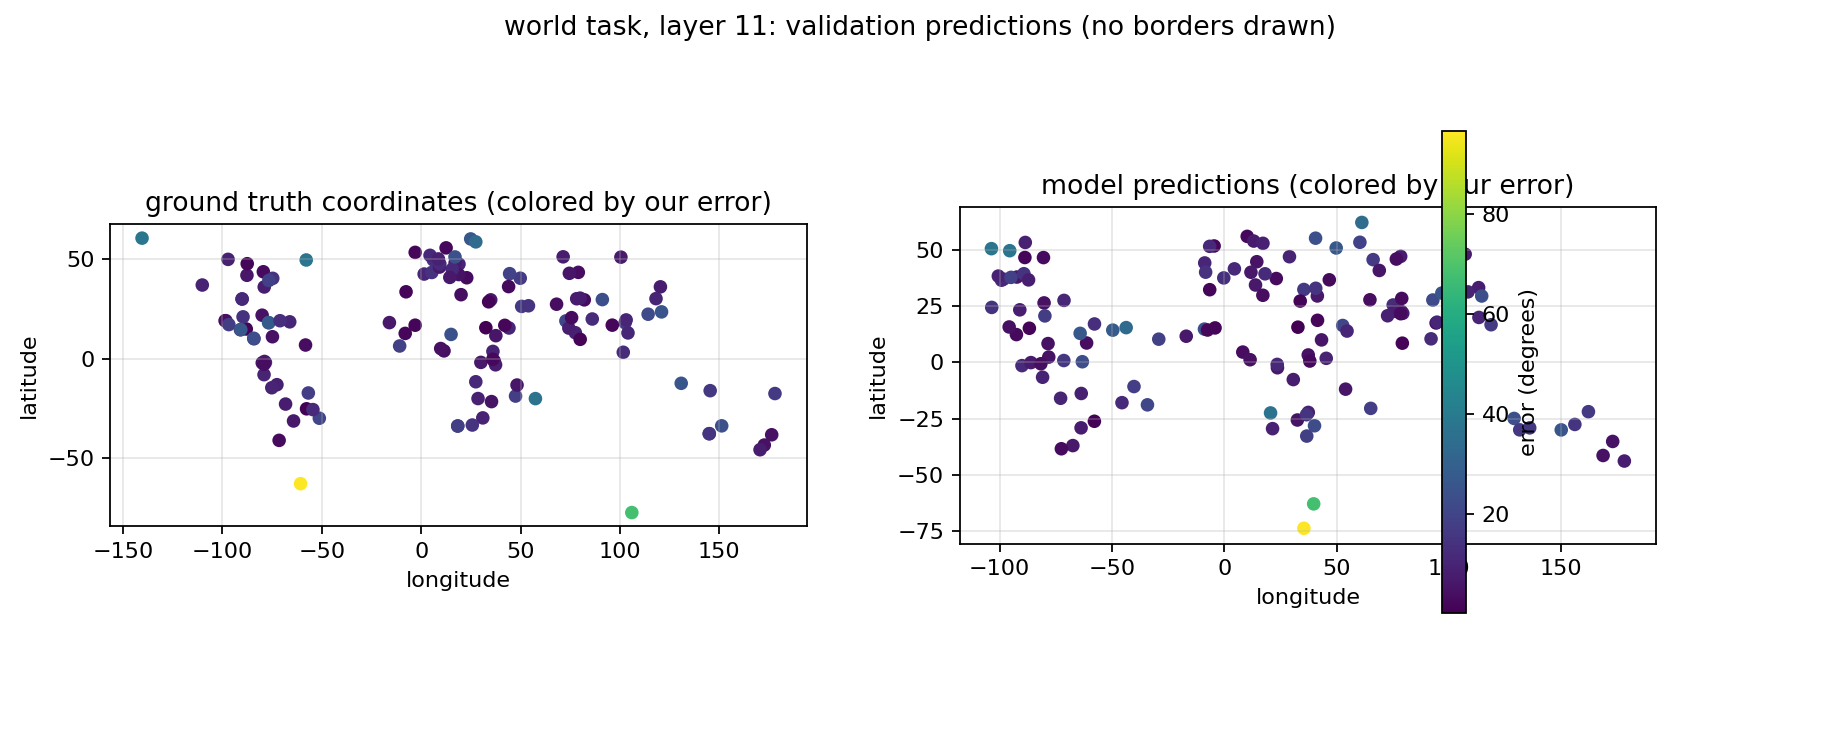
\includegraphics[width=0.48\textwidth]{figures/valid_predictions.png}
  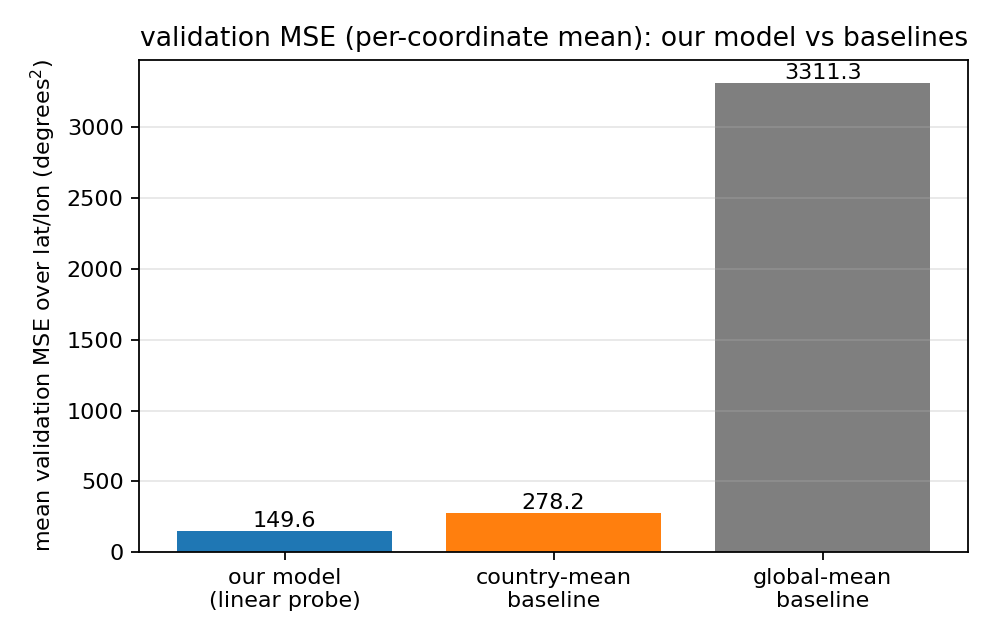
\includegraphics[width=0.48\textwidth]{figures/baseline_compare.png}
  \caption{左：130 条验证样本的预测坐标 vs 真实坐标（散点按误差着色）；
  右：我们的模型与两个基线的验证 MSE 对照（逐坐标平均 MSE）。}
\end{figure}

\paragraph{定量结果}
\begin{itemize}
  \item 我们模型在验证集上的\emph{总体} MSE 取两个坐标的逐坐标平均
  MSE $=149.64$；拆分看为纬度 MSE $=29.14$、经度 MSE $=270.13$
  （两者之和 $299.27$ 是\emph{“纬度 MSE + 经度 MSE”}，不是 MSE）；
  按等距近似折算平均大圆距离误差约 $1360$ km。
  \item 对照（同样为逐坐标平均 MSE）：全局均值基线 $3311.27$，
  按训练集国家分组的均值基线 $278.24$。
\end{itemize}

%-------------------------------------------------------------
\subsection{思考题 7：是否能说明模型内部存在地理坐标表征，而不只是识别国家}

\begin{figure}[htbp]
  \centering
  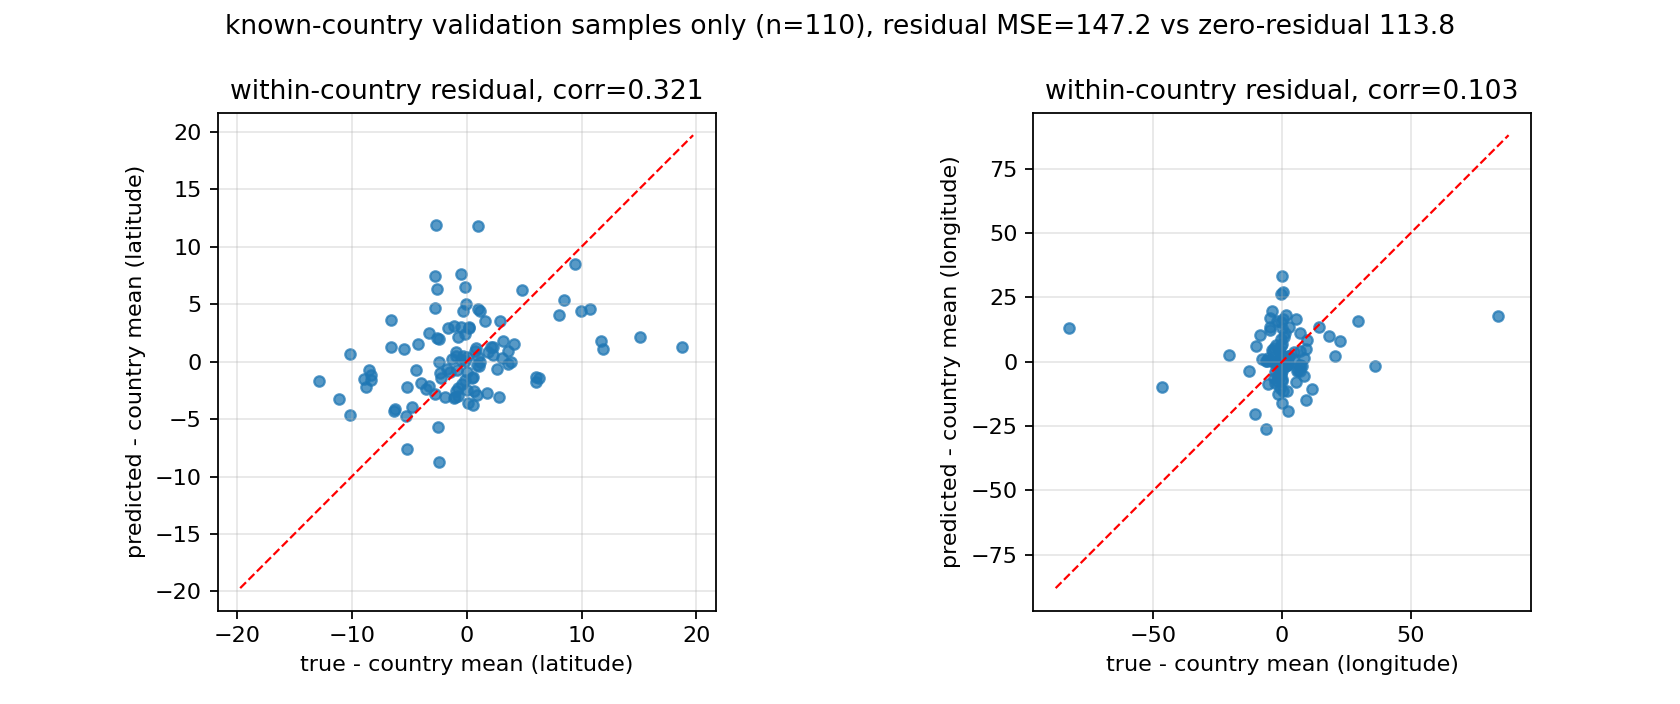
\includegraphics[width=0.62\textwidth]{figures/residual_vs_country.png}
  \caption{扣除训练集国家均值后的残差对照，\textbf{仅在训练集中出现过的国家的
  110 条验证样本上}评估：横轴为真实残差、纵轴为模型预测残差，红虚线为 $y=x$。
  若模型只“认国家”、不含国家内部坐标信息，散点应无相关且集中在 0 附近。}
\end{figure}

\begin{table}[htbp]
\centering
\caption{国家均值基线与本模型的分组对照（验证集 130 条；表中数值为逐坐标
平均 MSE，即纬度、经度两维 MSE 的平均）。}
\label{tab:country}
\begin{tabular}{lccc}
\toprule
分组 & 样本数 & 我们的模型 & 国家均值基线 \\
\midrule
全部验证样本 & 130 & \textbf{149.64} & 278.24（全局均值 3311.27） \\
训练集\emph{见过}的国家 & 110 & 147.21 & \textbf{113.77} \\
训练集\emph{未见}的国家 & 20 & \textbf{162.95} & 1182.83（退化为全局均值） \\
\midrule
\multicolumn{4}{l}{\emph{残差分析：仅在训练集见过的国家（110 条）上}} \\
残差预测误差 $\operatorname{mean}\big((\hat r-r)^2\big)$ & 110 & 147.21 & 113.77（$r$ 恒为 0 的基线） \\
残差相关系数（纬 / 经） & 110 & 0.321 / 0.104 & --- \\
\bottomrule
\end{tabular}
\end{table}

\paragraph{回答}
\textbf{证据是“部分支持、但不能单独成立”，需要与未见国家泛化合起来看。}
\begin{enumerate}
  \item \textbf{残差相关为正但明显偏弱}：把每条样本减去其所属国家在训练集中的
  平均坐标后，在训练集见过的 110 条上，模型预测残差与真实残差的相关系数为
  纬度 $0.321$、经度 $0.104$——存在同向变化的信号，但远未接近 1，
  且经度方向已很弱。若模型只识别国家、完全不含国家内部信息，这两个相关应接近 0。
  \item \textbf{但残差层面的误差并未优于“不预测”}：在同一 110 条上，
  模型残差预测误差 $\operatorname{mean}((\hat r-r)^2)=147.21$，
  而“残差恒为 0”（完全不预测国家内部偏移）的基线 $\operatorname{mean}(r^2)=113.77$。
  也就是说\textbf{模型给出的国家内部偏移反而使误差变大了}约 $33.4$
  （147.21 $-$ 113.77），所以“能预测国家内部坐标”并不能从残差 MSE 上得到支持，
  只能从残差相关上看到微弱的线性信号。
  \item \textbf{更强的证据来自未见国家泛化}：验证集中 20 条来自训练时未出现的国家，
  我们 MSE 162.95，而“按国家查表”的基线退化为全局均值（1182.83）。
  如果模型只会“认国家”，对未见国家就只能退化为常数预测、误差会很大；
  这里显著更优，说明表征里携带了可跨国家泛化的连续坐标信息。
  \item \textbf{反面证据}：在训练见过的 110 条上，国家均值基线（113.77）仍优于
  我们（147.21），说明在见过的国家里“查国家均值”已是非常强的预测，
  模型并未在国家内部把误差进一步压下去。
  \item 综合起来更审慎的表述是：\textbf{表征中既含国家级信息，也含可跨国家泛化的
  连续坐标信息}；后者主要由未见国家的泛化优势支持，而国家内部的残差证据
  （正相关）较弱、且残差 MSE 未超过零残差基线，不足以单独下结论。
  这与原文 Gurnee \& Tegmark (2024) 关于“语言模型线性表示空间”的结论方向一致
  （线性探测可解码空间信息），但本实验的残差分析并不支持更强的“精确内部坐标”说法。
\end{enumerate}

%-------------------------------------------------------------
\subsection{思考题 8：truth 训练/验证集的分布差异与应对}

脚本 \texttt{data\_analysis.py}（图 \ref{fig:dist_truth}）。

\begin{figure}[htbp]
  \centering
  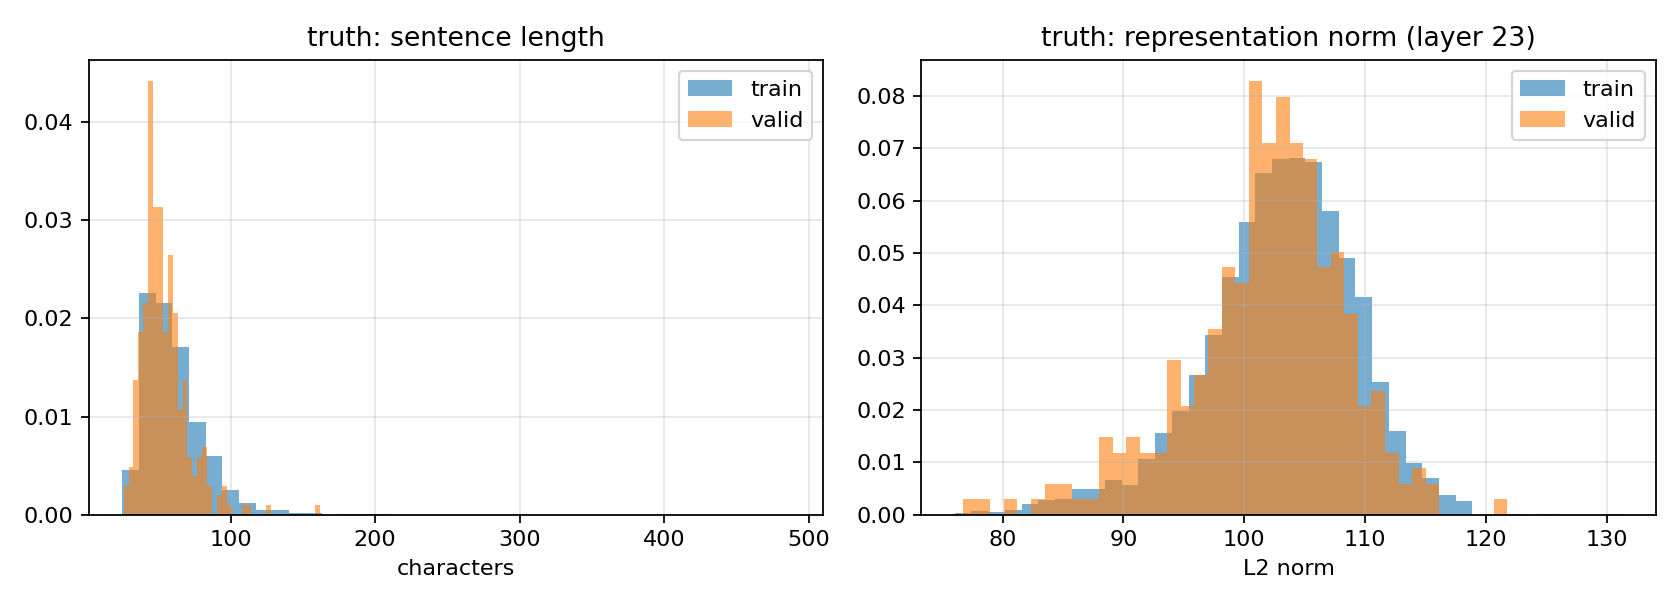
\includegraphics[width=0.78\textwidth]{figures/dist_truth.png}
  \caption{truth 训练/验证集分布对照：句长、表征范数与漂移、域分类器可分性。}
  \label{fig:dist_truth}
\end{figure}

\begin{table}[htbp]
\centering
\caption{truth 训练集与验证集的差异（显著性检验用双样本 KS 检验）。}
\label{tab:shift}
\small
\begin{tabular}{lc}
\toprule
统计量 & 数值（训练集 5088 / 验证集 300） \\
\midrule
正/负标签比例 & 0.5000 / 0.5000，两边均严格均衡 \\
句长均值（字符） & 60.95 vs 54.18（KS $p=3.0\times10^{-7}$） \\
词数均值 & 10.32 vs 9.32（KS $p=5.1\times10^{-5}$） \\
第 23 层表征范数 & $102.94\pm6.30$ vs $101.75\pm6.63$（KS $p=0.028$） \\
逐维均值漂移（按逐维 std 归一） & 0.128 / 0.121 / 0.136（第 11/23/35 层） \\
域分类器区分 train/valid 的测试准确率（第 23 层） & \textbf{0.9332}（0.5 表示不可区分） \\
\bottomrule
\end{tabular}
\end{table}

\paragraph{差异}两类数据的\textbf{标签都是严格 50/50 均衡}，不存在标签偏移；
差异主要在\textbf{输入（句长）与表征分布}：验证集句子显著更短，
域分类器仅凭第 23 层表征就能以 93.3\% 的准确率区分训练/验证样本，
说明差异是线性可检出的、真实存在的。

\paragraph{应对}
\begin{enumerate}
  \item \textbf{正则化 + 早停}：$\lambda_2$ 把训练准确率从 0.9988 压到 0.9381，
  验证准确率从 0.8567 提升到 0.8833，直接缩小泛化差距。
  \item \textbf{按长度分桶定位差距来源}（最终模型，第 23 层）：
  验证集 $<55$ 字符准确率 $0.857$（$n=182$）、55--65 字符 $0.936$（$n=62$）、
  $>65$ 字符 $0.911$（$n=56$）；训练集对应为 $0.932/0.944/0.943$。
  可见短句更难，而验证集里短句占比 61\%（训练集 47\%）——
  若按训练集句长分布重新加权，验证准确率约 $0.894$，
  即\textbf{约 1 个点的差距来自句长组成变化}，其余约 4 个点是真实泛化差距。
  这也解释了为什么总准确率（0.8833）看起来比训练准确率（0.9381）低很多。
  \item \textbf{不做依赖句长的特征工程或增广}，避免把“长度”这一分布差异
  当作捷径学进权重里；预测只用第 23 层表征，不引入句长等表面特征。
  \item \textbf{调参保守}：层数与 $\lambda$ 虽然在验证集上选，但都选在
  平台区（$\lambda_2\in[0.02,0.05]$ 准确率均为 $0.877\sim0.883$）而非尖点，
  以降低在 300 条验证集上过拟合的风险；
  同时用 \texttt{sklearn} 独立复核（见思考题 3），确认该解就是同一目标函数的最优解，
  而非偶然的局部好点。
  \item \textbf{如实承认}：仍有约 4 个点的真实泛化差距，且验证集小、
  被用于选层选参，存在一定的选择偏差；报告中的分桶结果可用于验收时解释。
\end{enumerate}

%-------------------------------------------------------------
\subsection{思考题 9：truth 最终提交的选层与选正则}

\begin{table}[htbp]
\centering
\caption{truth 任务：各层调参后的最好结果（粗网格 + 细网格，共 11 个 $\lambda$/层）。}
\label{tab:layer_truth}
\begin{tabular}{lcccc}
\toprule
层 & 最优 $\lambda_2$ & 验证准确率 & 训练准确率 & $\lambda_2=0$ 时验证准确率 \\
\midrule
11 & 0.01 & 0.7533 & 0.8239 & 0.7067 \\
\textbf{23} & \textbf{0.03} & \textbf{0.8833} & \textbf{0.9381} & 0.8567 \\
35 & 任意（0 即可） & 0.8167 & 0.9809 & 0.8167 \\
\bottomrule
\end{tabular}
\end{table}

\paragraph{选层理由}
\begin{enumerate}
  \item 验证准确率上第 23 层（0.8833）显著优于第 11 层（0.7533）与第 35 层
  （0.8167），差距达 7--13 个百分点。
  \item 从表征本身也能预测这一结果：第 23 层与标签相关性最强的特征
  $|r|_{\max}=0.376$、$|r|>0.1$ 的特征有 1141 个，而第 11/35 层分别只有
  180/572 个（$|r|_{\max}=0.196/0.275$），即“真假”信息在第 23 层最线性可解码。
  \item 第 35 层不加正则与加正则结果完全一样（都是 0.8167）且训练准确率
  0.9809，说明它既没有更强的信号、又更容易过拟合。
\end{enumerate}

\paragraph{选正则理由}
\begin{enumerate}
  \item 只用 $\ell_2$，$\lambda_2$ 粗网格 $\{0,10^{-5},10^{-4},10^{-3},0.01,0.1\}$
  后细网格 $\{0.005,0.02,0.03,0.04,0.05\}$；
  验证准确率随 $\lambda_2$ 单调上升到平台：
  $0.8567\ (\lambda=0)\to0.8633\ (10^{-3})\to0.8733\ (0.005\text{--}0.01)
  \to0.8767\ (0.02)\to0.8833\ (0.03,0.04,0.05)\to0.8700\ (0.1)$。
  \item 取平台中较早的 $\lambda_2=0.03$（平台 $[0.02,0.05]$ 内三点同为 0.8833，
  取值不敏感），对应训练准确率从 0.9988 降到 0.9381，说明确实抑制了过拟合
  而非单纯拟合验证集。
  \item 用 \texttt{sklearn} 交叉验证换算 $C=1/(2N\lambda_2)=0.00328$，
  得到同样的 0.8833、$\cos(w)=0.999999$，说明该 $\lambda$ 对应的是
  目标函数的全局最优，不是手写 GD 的偶然结果。
  \item 因为验证集只有 300 条，$\lambda$ 取平台内部而非边缘，
  并保留 $\ell_2$ 而非 $\ell_1$（任务是分类预测，稀疏性无收益）。
  \item 训练配置本身也是一种“隐式正则”，单独考察过：
  动量 $0.99/8000$ 步、普通 GD $20000$ 步（含不同 patience）、
  普通 GD + 学习率衰减，$\times$
  $\lambda_2\in\{0,0.01,0.03,0.05\}$ 共 16 组。
  普通 GD 收敛慢（2 万步仍欠收敛，训练准确率仅 0.9312）
  相当于隐式早停，在官方验证集上 $\lambda_2=0$ 可到 0.8867，
  但只比 0.8833 多 1 条样本。
  为避免在 300 条验证集上反复择优，把训练集内部再切 10\% 复核
  （4580/508，固定随机种子）：内部验证集上本配置最好（0.9016），
  普通 GD 的 $\lambda_2=0/0.01/0.03$ 分别为 0.8976/0.8976/0.8957，
  故最终仍提交“动量 $0.99$ + $\lambda_2=0.03$”。
\end{enumerate}

\paragraph{提交物}
\begin{itemize}
  \item \texttt{results/world.npz}：\texttt{weights} 形状 $(2,2560)$、
  \texttt{bias} 形状 $(2,)$，类型 \texttt{float64}；层数 \textbf{11}。
  \item \texttt{results/truth.npz}：\texttt{weights} 形状 $(2560,)$、
  \texttt{bias} 形状 $()$，\texttt{float64}；层数 \textbf{23}。
\end{itemize}

%=============================================================
\newpage
\appendix

\section{复现方式与代码位置}

核心代码位置（未使用 \texttt{sklearn} 的拟合接口完成训练）：
\begin{itemize}
  \item \texttt{model.py}：线性回归 / 逻辑回归的全批量梯度下降
  （$\ell_1$ 次梯度、$\ell_2$ 正则、幂迭代自动学习率、可选动量与学习率衰减、
  基于损失的早停），对应讲义 2.1 节全部公式；偏置不参与正则。
  \item \texttt{train1.py} / \texttt{train23.py}：助教框架下的训练入口。
  \item \texttt{sweep.py}：world/truth 的层数与 $\lambda$ 粗细网格搜索，
  并写出 \texttt{results/*.npz}。
  \item \texttt{coef\_path.py}、\texttt{feature\_selection\_demo.py}、
  \texttt{compare\_sklearn.py}：思考题 1--3。
  \item \texttt{data\_analysis.py}、\texttt{plot\_maps.py}：思考题 6--8 的
  分析与可视化。
\end{itemize}

复现命令（在 \texttt{LABs/LAB1} 下）：
\begin{verbatim}
python train1.py
python sweep.py                    # 粗+细网格，产出 results/*.npz
python coef_path.py                # 图 1
python feature_selection_demo.py   # 图 2
python compare_sklearn.py          # 表 3
python data_analysis.py            # 图 3（分布差异）
python plot_maps.py                # 图 4--6（地图可视化与基线）
\end{verbatim}

\section{主要实验记录}

\begin{table}[htbp]
\centering
\caption{world：第 11 层 $\lambda_2$ 与验证集指标（细网格标注为“细”）。
“纬度 MSE + 经度 MSE”列为两项 MSE 之和，不是 MSE。}
\begin{tabular}{lcccl}
\toprule
$\lambda_2$ & 纬度 MSE & 经度 MSE & 纬度 MSE + 经度 MSE & 阶段 \\
\midrule
0      & 75.643 & 713.531 & 789.17 & 粗 \\
0.001  & 68.582 & 670.110 & 738.69 & 粗 \\
0.01   & 44.491 & 500.711 & 545.20 & 粗 \\
0.05   & 31.188 & 345.138 & 376.33 & 粗 \\
0.07   & 29.998 & 320.862 & 350.86 & 细 \\
0.1    & 29.296 & 299.970 & 329.27 & 粗 \\
0.14   & \textbf{29.141} & 285.099 & 314.24 & 细 \\
0.2    & 29.497 & 274.676 & 304.17 & 粗 \\
0.28   & 30.329 & \textbf{270.130} & 300.46 & 细 \\
0.4    & 31.785 & 271.348 & 303.13 & 细 \\
0.5    & 33.047 & 275.587 & 308.63 & 粗 \\
1      & 39.411 & 309.883 & 349.29 & 粗 \\
\midrule
\multicolumn{4}{l}{最终取纬度 $\lambda=0.14$、经度 $\lambda=0.28$，“纬度 MSE + 经度 MSE” $=$ \textbf{299.27}} & \\
\bottomrule
\end{tabular}
\end{table}

\begin{table}[htbp]
\centering
\caption{truth：第 23 层 $\lambda_2$ 与准确率。}
\begin{tabular}{lcc}
\toprule
$\lambda_2$ & 训练准确率 & 验证准确率 \\
\midrule
0      & 0.9988 & 0.8567 \\
0.001  & 0.9963 & 0.8633 \\
0.005  & 0.9752 & 0.8733 \\
0.01   & 0.9619 & 0.8733 \\
0.02   & 0.9465 & 0.8767 \\
\textbf{0.03} & 0.9381 & \textbf{0.8833} \\
0.04   & 0.9306 & 0.8833 \\
0.05   & 0.9261 & 0.8833 \\
0.1    & 0.9121 & 0.8700 \\
\bottomrule
\end{tabular}
\end{table}

\paragraph{训练配置补充实验}
原始记录见 \texttt{results/opt\_sweep.txt}、\texttt{results/tiebreak.txt}。
truth 上比较 4 种配置（动量 $0.99/8000$ 步、普通 GD $20000$ 步
patience 50/200、普通 GD+学习率衰减）$\times$
$\lambda_2\in\{0,0.01,0.03,0.05\}$；
world 第 11 层上比较 3 种配置 $\times$ $\lambda_2\in\{0.14,0.2,0.28,0.4\}$。
world 结果：同一 $\lambda$ 下三种配置的“纬度 MSE + 经度 MSE”相差不到 1\%
（如 $\lambda=0.28$：300.46 / 300.45 / 300.15），
且都劣于“纬度、经度各自取 $\lambda$”的 299.27，故不更换配置。
truth 结果与内部切分复核见思考题 9 第 4 点。

\section{实现过程中的问题与解决}

\begin{enumerate}
  \item \textbf{闭式解核对差一个 2 倍}：一度用
  $(X^\top X/N+2\lambda_2 I)^{-1}$ 当参考解，与 GD 结果总差 $3\times10^{-2}$。
  按讲义目标 $\text{mean}(r^2)+\lambda_2\|w\|^2$ 重新求导应为
  $(X^\top X/N+\lambda_2 I)$，改用 $1\times$ 后偏差降到 $10^{-16}$，
  说明 \texttt{model.py} 实现正确、参考解写错了。
  \item \textbf{次梯度无法得到精确 0}：固定步长的次梯度法在零点附近振荡，
  $\lambda$ 很大时损失仍停在 2.3（最优 1.0）。系数路径与稀疏案例改用 ISTA
  得到精确稀疏解，\texttt{model.py} 保持次梯度（符合讲义要求）。
  \item \textbf{\texttt{sklearn} 接口}：\texttt{LinearRegression} 没有
  \texttt{alpha}，岭回归应使用 \texttt{Ridge}；
  二分类的 \texttt{coef\_ shape} 是 $(1,D)$，需 \texttt{ravel()} 后再比较。
  \item \textbf{全批量 GD 在原始特征上收敛慢}：$N=500\ll D=2560$ 且特征均值
  非零时存在近零曲率方向，60 万步仍有 $0.14$ 的目标差；
  标准化后同一 GD 收敛到与 \texttt{sklearn} 完全一致的解（$10^{-14}$）。
\end{enumerate}

\section{实验反馈与建议}

\begin{itemize}
  \item 文档对 world 任务提示“测试集分布更接近验证集”，
  但未说明验证集有多少条；建议补充验证集/测试集规模，
  便于判断 $\lambda$ 网格搜索的可信区间。
  \item 建议提供一个官方的评估脚本或基线数值（如全局均值、国家均值），
  方便同学自查；本次的国家均值基线是自己实现的，与文档描述的
  “按训练集国家分组的平均坐标基线”一致。
  \item 附录 B 的算力平台教程对非计算机专业同学门槛略高，
  建议给出可直接运行的 \texttt{sbatch} 模板与常见报错示例。
\end{itemize}

\end{document}
